\chapter{System Design and Data Design}
\label{chap:system_design_data}

This chapter presents the system design and data design of the Horse Racing Tournament Management System. The main purpose of this chapter is to describe the database structure and the object-oriented design of the system.

The system design is based on the main business workflow, including user management, horse management, tournament management, race scheduling, jockey invitation, result recording, ranking update, and spectator view.

\section{Entity Relationship Diagram}

The Entity Relationship Diagram describes the main data entities of the system and the relationships among them. It helps the development team understand how data is stored and connected in the database.

Figure~\ref{fig:erd} shows the Entity Relationship Diagram of the Horse Racing Tournament Management System.

\begin{figure}[H]
	\centering
	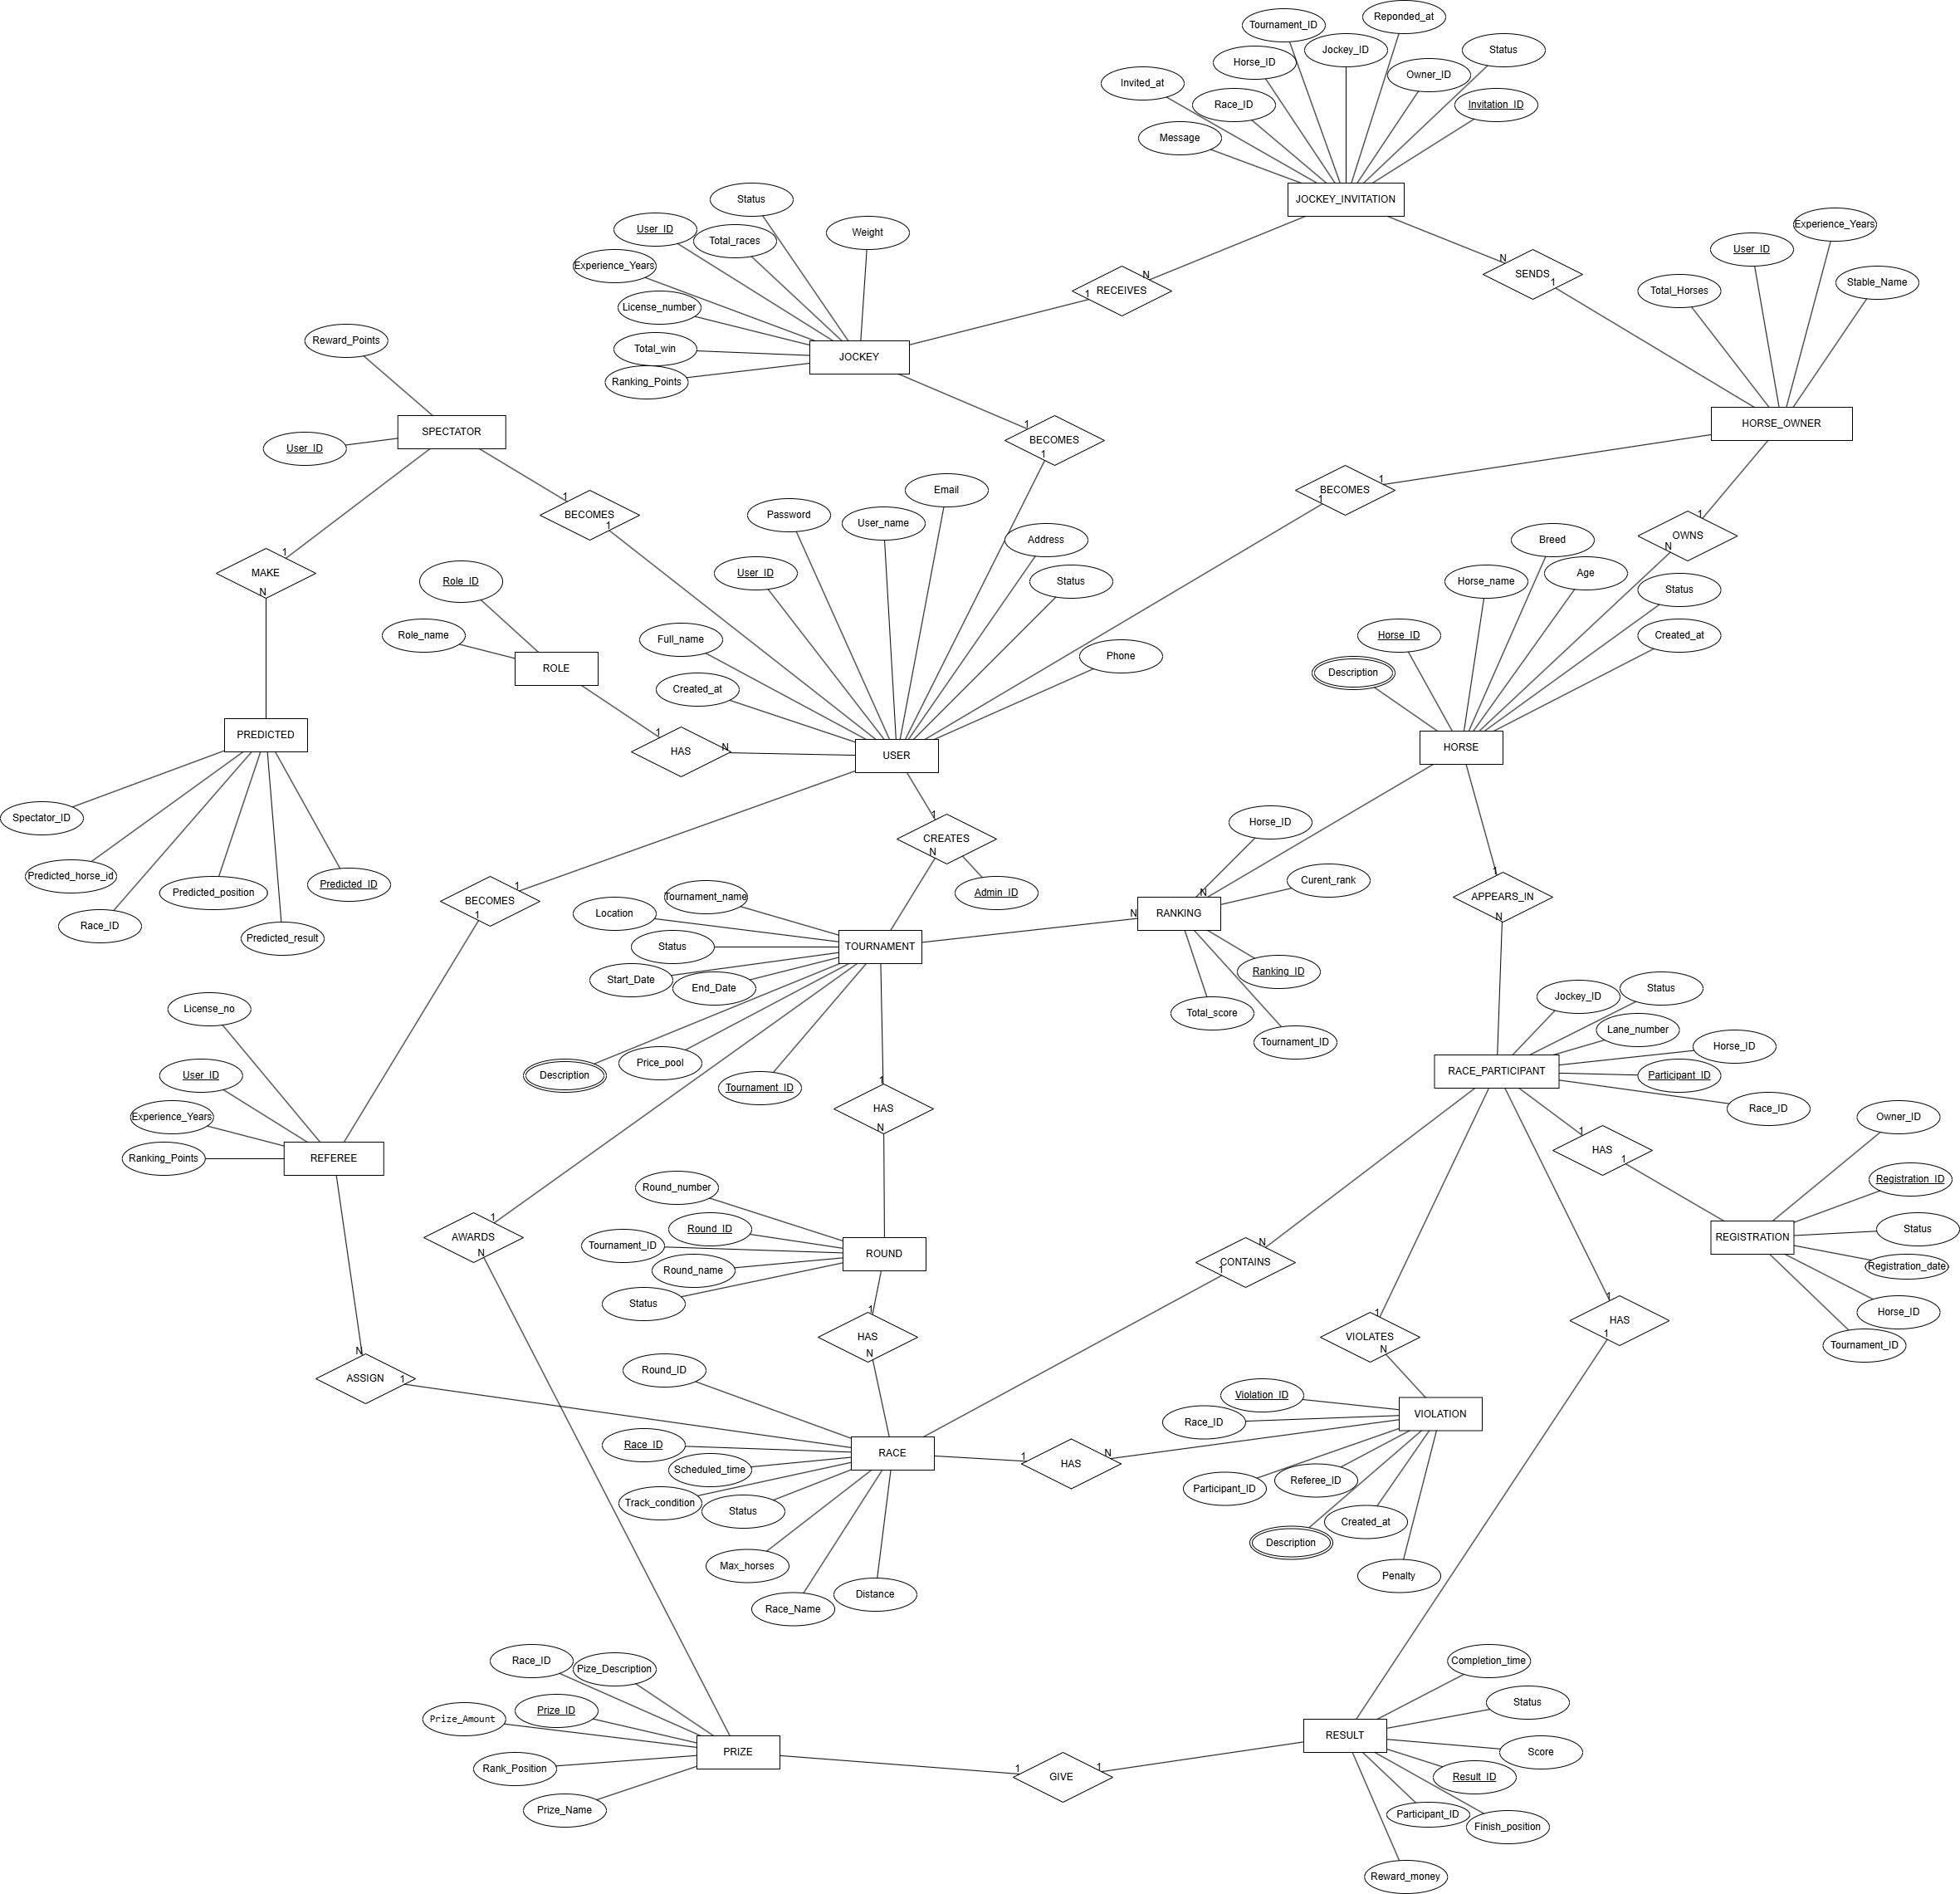
\includegraphics[width=0.90\textwidth,height=0.60\textheight,keepaspectratio]{images/chuong4/ERD.png}
	\caption{Entity Relationship Diagram of the Horse Racing Tournament Management System}
	\label{fig:erd}
\end{figure}

\subsection{Main Entities}

The system includes several important entities. The User entity stores account information for all users in the system. Each user has a role such as Admin, Horse Owner, Jockey, Referee, or Spectator.

The Horse entity stores information about horses, including horse name, breed, age, status, and owner. A Horse Owner can manage many horses and register them for tournaments.

The Tournament entity stores information about horse racing tournaments. Each tournament may contain several rounds and races. The Race entity stores the race schedule, race distance, track condition, and race status.

The Registration entity stores registration requests from Horse Owners. A registration must be approved before a horse can join a race.

The Jockey Invitation entity stores invitations sent from Horse Owners to Jockeys. A Jockey can accept or decline an invitation.

The Race Participant entity connects a race with its participating horse and jockey. This entity is used to manage the official participant list of each race.

The Result entity stores race results, including finish position, completion time, score, and result status. The Ranking entity stores ranking information based on confirmed race results.

The Violation entity stores violation records during a race. The Prize entity stores prize information for race winners. The Prediction entity stores spectator predictions.

\subsection{Main Relationships}

The User entity is connected to the Role entity to support role-based access control. A Horse Owner can own many horses, while each horse belongs to one owner.

A Tournament can contain many Rounds, and each Round can contain many Races. This structure allows the Admin to organize the tournament clearly.

A Horse Owner submits a Registration for a horse to join a tournament. After the registration is approved, the horse can be assigned to a race.

A Horse Owner can send a Jockey Invitation to a Jockey. When the invitation is accepted, the system can assign the horse and jockey as race participants.

Each Race can have many Race Participants. After the race is completed, each participant receives a Result. Confirmed results are then used to update the Ranking.

Referees can record Violations and confirm race results. Spectators can view public race information and submit Predictions.

\subsection{Data Constraints}

The database must maintain data consistency. Each record should have a primary key, and related records should be connected using foreign keys.

The system should only allow approved registrations to be assigned to races. A horse should not be assigned to two races at the same time. A jockey should not be assigned to conflicting race schedules.

Race results should only be used to update rankings after they are confirmed by the Referee or Admin.

\section{Class Diagram}

The Class Diagram describes the main classes of the system and how they interact with each other. It represents the object-oriented structure of the Horse Racing Tournament Management System.

Figure~\ref{fig:class_diagram} shows the Class Diagram of the system.

\begin{figure}[H]
	\centering
	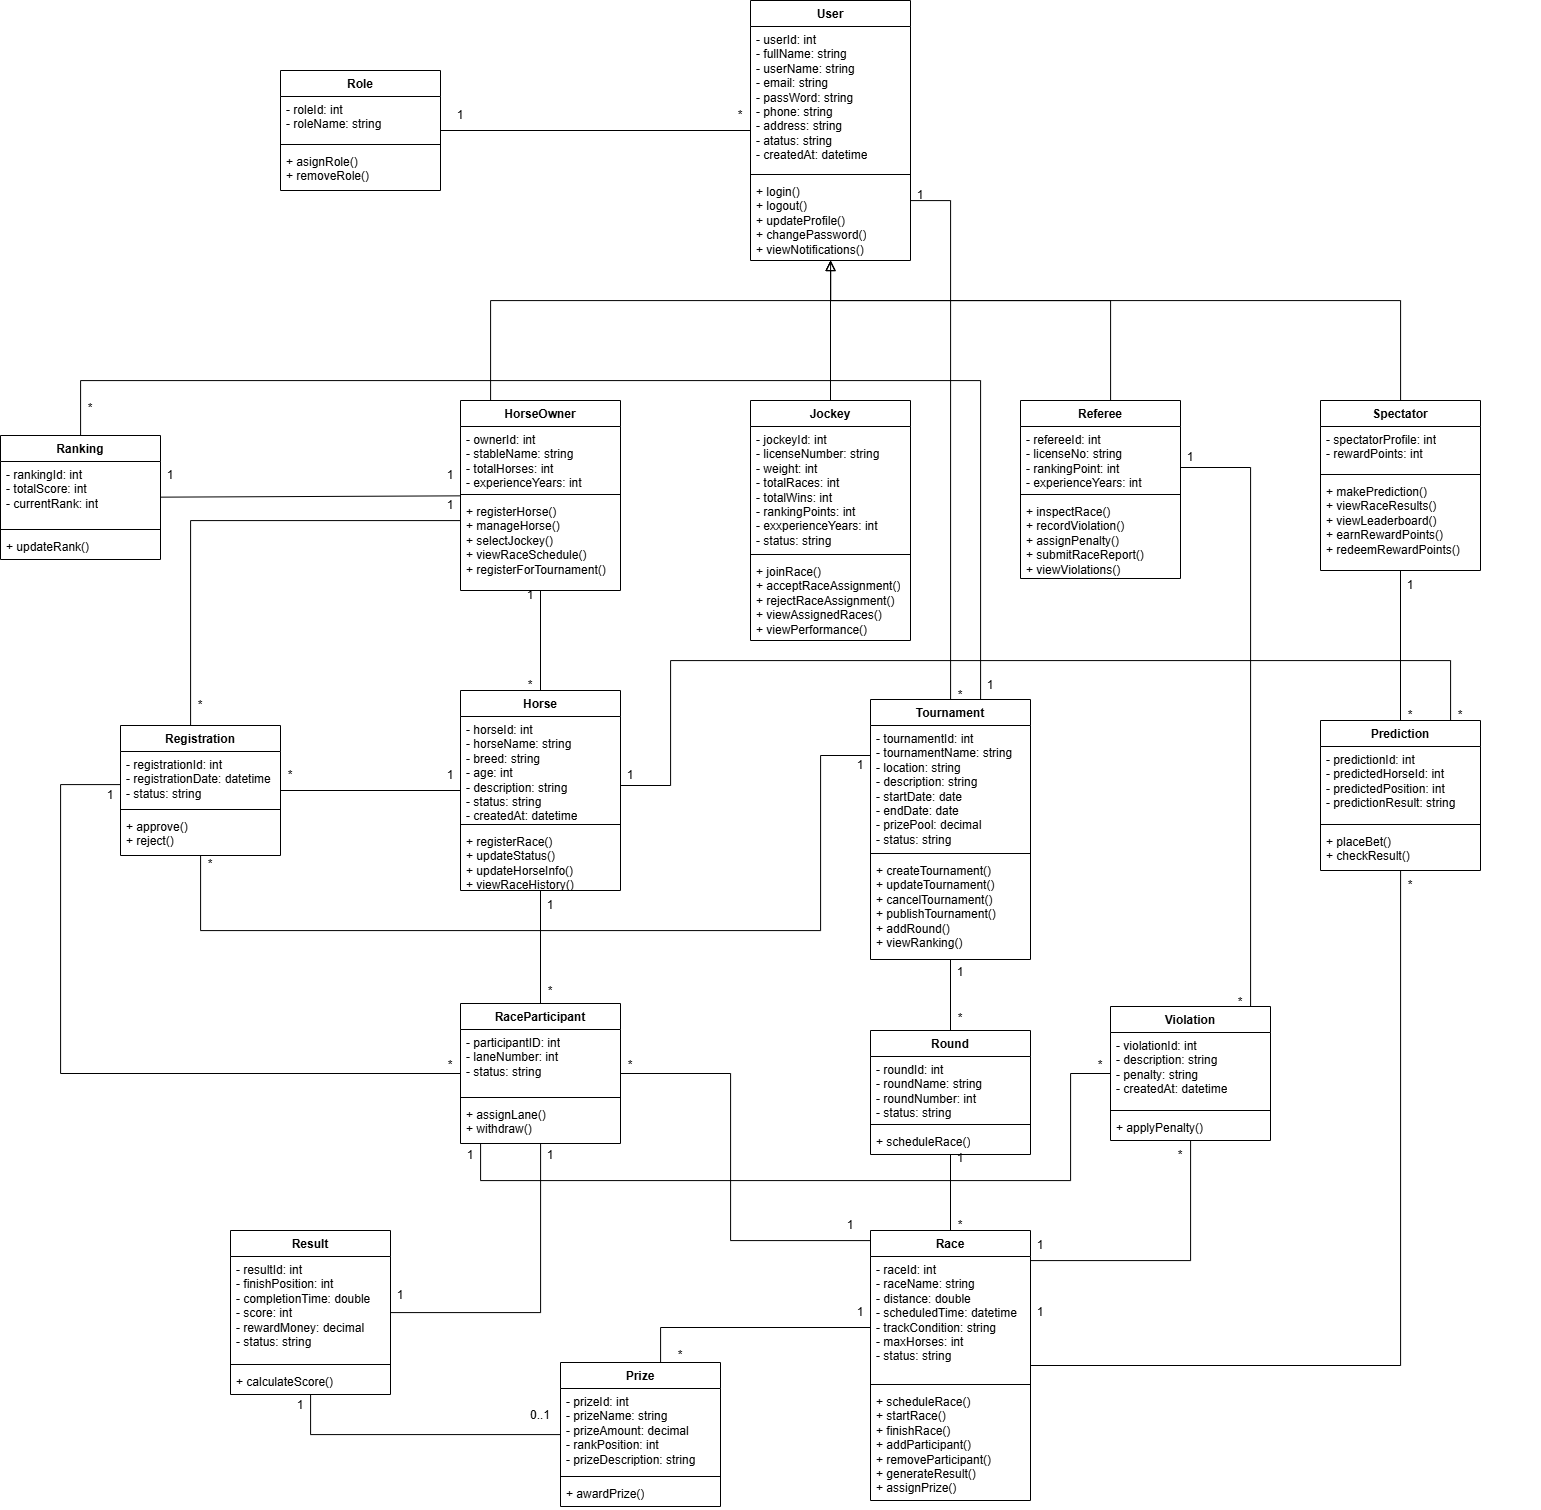
\includegraphics[width=0.90\textwidth,height=0.60\textheight,keepaspectratio]{images/chuong4/class_diagram.png}
	\caption{Class Diagram of the Horse Racing Tournament Management System}
	\label{fig:class_diagram}
\end{figure}

\subsection{Main Classes}

The User class represents a general user account in the system. It contains common information such as username, password, full name, email, phone number, and role.

The HorseOwner class represents the user who owns and manages horses. This class supports horse management, tournament registration, jockey invitation, schedule viewing, and result tracking.

The Jockey class represents the user who rides horses in races. This class supports accepting or declining invitations and viewing assigned races.

The Referee class represents the user who checks races, records violations, and confirms race results.

The Spectator class represents the user who views public tournament information, race schedules, results, rankings, and predictions.

The Horse class represents a horse in the system. It stores horse information and supports race registration.

The Tournament class represents a horse racing tournament. It manages tournament information, rounds, races, and ranking.

The Race class represents a specific race. It manages schedule information, participants, results, and race status.

The Registration class represents a horse registration request. It supports approval and rejection.

The RaceParticipant class connects a horse, a jockey, and a race. It represents one official participant in a race.

The Result class stores race result information. It supports score calculation and result confirmation.

The Ranking class stores leaderboard information and updates ranking based on confirmed results.

The Violation class stores race violation information. The Prize class stores prize information. The Prediction class stores spectator prediction information.

\subsection{Design Explanation}

The system uses a role-based design. The User class stores common account information, while specific roles such as HorseOwner, Jockey, Referee, and Spectator provide role-specific functions.

The main business classes are Tournament, Race, Registration, RaceParticipant, Result, and Ranking. These classes represent the main workflow of the system from tournament creation to result publication.

First, the Admin creates a tournament and races. Then, Horse Owners register horses for the tournament. After registration is approved, a horse and jockey can be assigned to a race. When the race is completed, the Referee records and confirms the result. The system then updates the ranking.

\section{Mapping Between Data Design and Class Design}

The ERD and Class Diagram are closely related. The ERD focuses on database structure, while the Class Diagram focuses on software structure.

The User entity maps to the User class. The Horse entity maps to the Horse class. The Tournament entity maps to the Tournament class. The Race entity maps to the Race class. The Registration entity maps to the Registration class. The Result entity maps to the Result class. The Ranking entity maps to the Ranking class.

This mapping helps the development team implement backend models, services, repositories, and APIs more consistently.

\section{Chapter Summary}

This chapter presented the system design and data design of the Horse Racing Tournament Management System. The ERD describes the main database entities and relationships. The Class Diagram describes the main classes and their responsibilities.

These designs provide a foundation for implementing the database, backend models, business logic, and system functions.
